\begin{figure}[h]
    \centering
    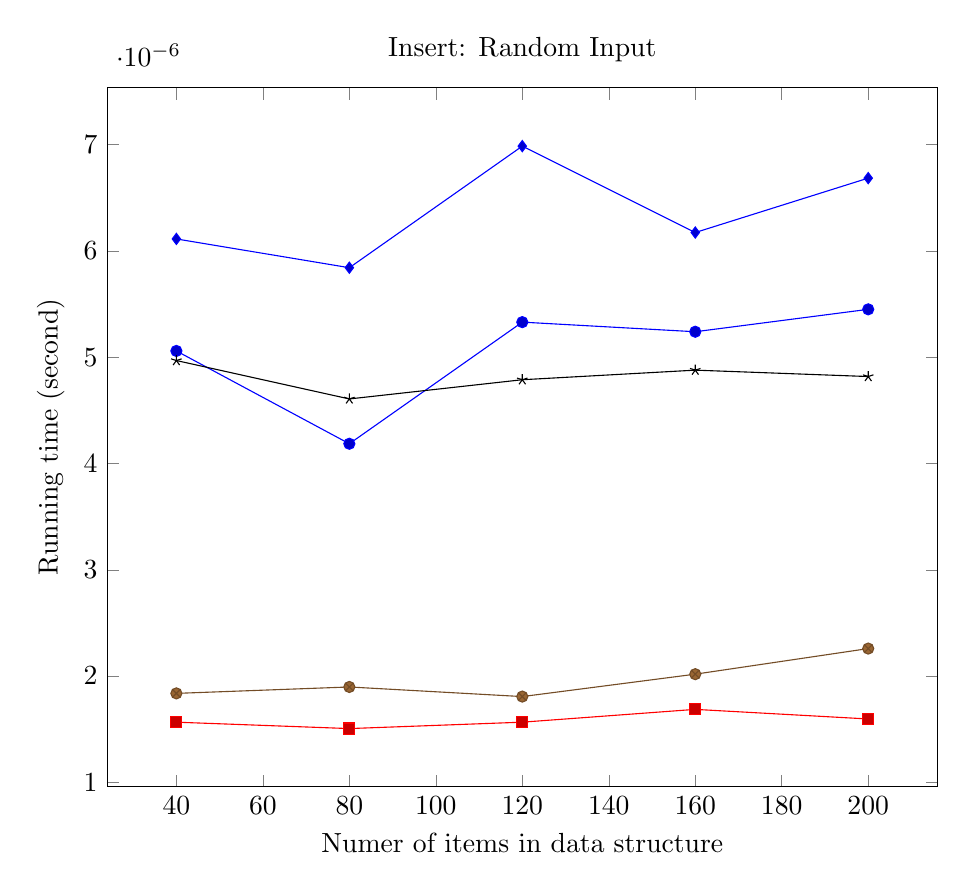
\begin{tikzpicture}
        \begin{axis}[
            xlabel={Numer of items in data structure},
            ylabel={Running time (second)},
            title={Insert: Random Input},
            width=\textwidth
        ]
		\addplot coordinates {
			(40, 5.059745657476355e-06)
			(80, 4.186337180911437e-06)
			(120, 5.330803460523726e-06)
			(160, 5.240450859744783e-06)
			(200, 5.4512735953693435e-06)
		};
		\addplot coordinates {
			(40, 1.566111751216681e-06)
			(80, 1.505876683793872e-06)
			(120, 1.566111751216681e-06)
			(160, 1.686581885707028e-06)
			(200, 1.5962292849280857e-06)
		};
		\addplot coordinates {
			(40, 1.8371695539087795e-06)
			(80, 1.89740462168686e-06)
			(120, 1.8070520205526463e-06)
			(160, 2.017874756177207e-06)
			(200, 2.2588150255131724e-06)
		};
		\addplot coordinates {
			(40, 4.9693930566974135e-06)
			(80, 4.607982652160558e-06)
			(120, 4.7886878540737145e-06)
			(160, 4.879040455207928e-06)
			(200, 4.818805388140391e-06)
		};
		\addplot coordinates {
			(40, 6.113859336309701e-06)
			(80, 5.842801533262332e-06)
			(120, 6.987267812519349e-06)
			(160, 6.17409440337724e-06)
			(200, 6.686092476115846e-06)
		};
        \legend{}
        \end{axis}
    \end{tikzpicture}
    \caption{Average of 0 operations, benchmarked every 0, starting at 0.}
\end{figure}